\documentclass[aspectratio=169,hyperref={pdfpagelabels=false}]{beamer}
\input{preamble.tex}
\usepackage{tikz}
\usepackage[siunitx]{circuitikz}
\usepackage{bm}
\usepackage{amsmath}
\usepackage{minted}

\usetikzlibrary{shapes.geometric, arrows, positioning}

\subtitle{\normalsize{Industrial IoT for Digitization of Electronis Assets}}
\title{}

\setdepartment{DTU Wind and Energy System}
\setcolor{blue}

\begin{document}
\inserttitlepage

%SLIDE 0
\begin{frame}{Agenda}
  \tableofcontents
\end{frame}

% SLIDE 1
\begin{frame}{Model Types}
  \begin{figure}[t]
    \centering
    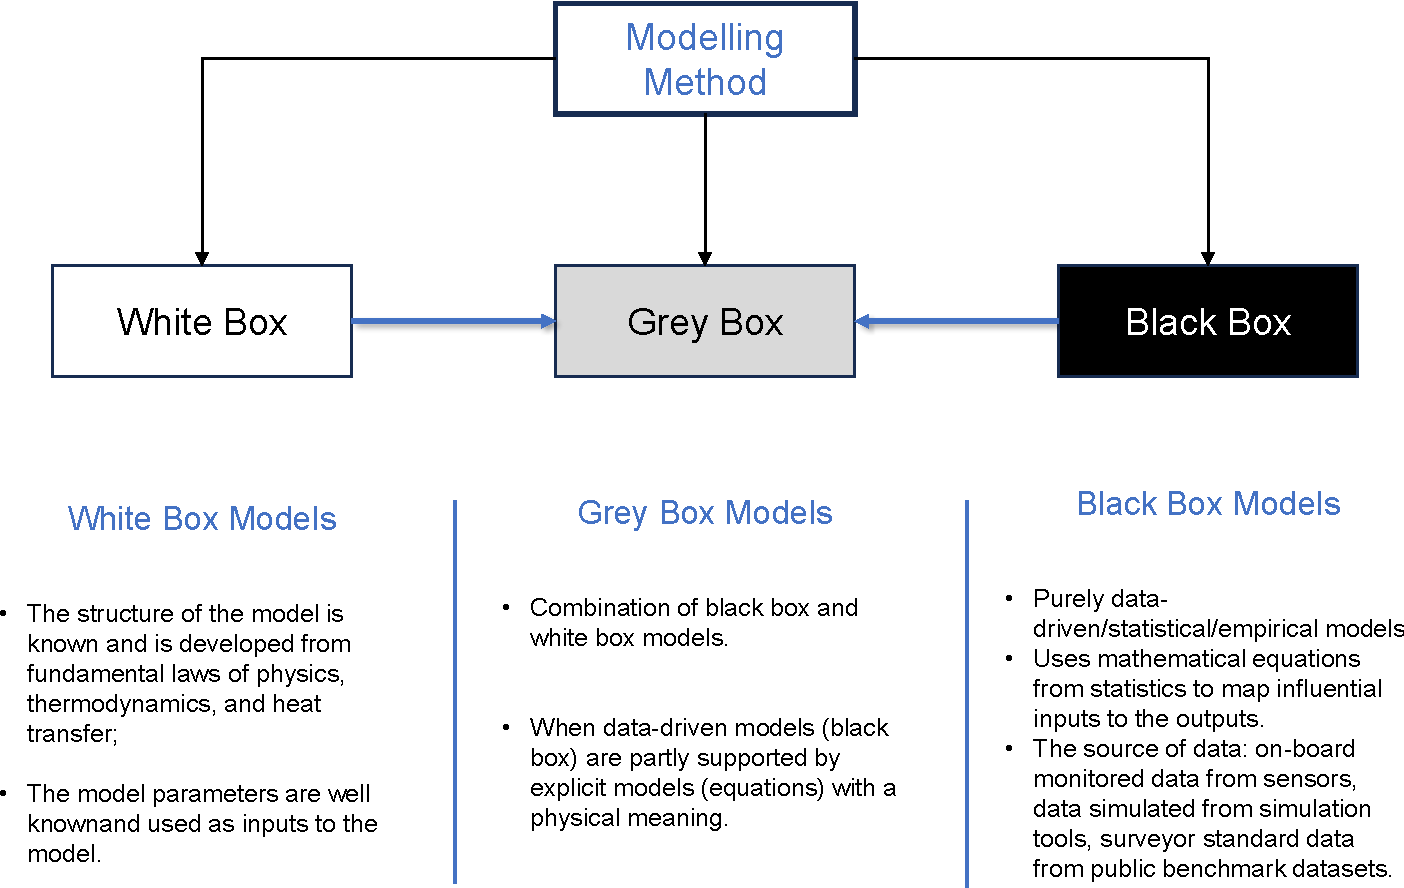
\includegraphics[width=0.85\textwidth]{img/modelling_methods.pdf}
\end{figure}
\end{frame}

% SLIDE 2
\begin{frame}{Example of White Box Model}
  We know the physics, so
  we can write the equations: 
  \begin{columns}
    \begin{column}{0.4\textwidth}
      \begin{circuitikz}
        \draw
        (0,0) -- (0,1)
        (0,3) -- (0,2)
        to[open] (0,3) % Open circuit (gap) instead of voltage source
        to[R, l=$R_0$] (2,3) -- (4,3)
        to[R, l=$R_1$] (4,0) -- (0,0)
        (2,3) -- (2,2)
        (2,2) -- (2,3)
        to[C, l=$C$] (2,0);
    
        \draw(0,1) -- (0.5,1.8);
        \node at (-0.4,1.9) {$+$};
        \node at (-0.4,1.4) {$V$};
        \node at (-0.4,0.9) {$-$};
        \draw[->,thick] (0.5,0.9) to[bend right] (0,1.5);
        \node at (0.7,0.6) {{\small\textit{$t>0$}}};
    \end{circuitikz}
  \end{column}
  \begin{column}{0.6\textwidth}

  \begin{tcolorbox}[width=1\linewidth, height = 0.4\linewidth]
    \textbf{\bm{$t \geq 0$}}\centering
    \begin{align*}
      I &= \frac{1}{R_1}V_{C} + C\frac{d}{dt}V_{C} \\
      V &= R_{0}I+ V_{C}\\
    \end{align*}
  \end{tcolorbox} \pause 
   
    \begin{tcolorbox}[width=1\linewidth, height = 0.3\linewidth]
      \textbf{\bm{$t \geq 0$}}\centering
      \begin{align*}
        V + CR_{1}\frac{d}{dt}V = (R_0 + R_1)I + CR_{0}R_{1}\frac{d}{dt}I
      \end{align*}
    \end{tcolorbox}
  \end{column}
  \end{columns}
\end{frame}

% SLIDE 3
\begin{frame}{Example of White Box Model}
The differential equation can be solved analitically, thus finding $I$ has an exponential reponse
  \begin{columns}
    \begin{column}{0.4\textwidth}
      \begin{circuitikz}
        \draw
        (0,0) -- (0,1)
        (0,3) -- (0,2)
        to[open] (0,3) % Open circuit (gap) instead of voltage source
        to[R, l=$R_0$] (2,3) -- (4,3)
        to[R, l=$R_1$] (4,0) -- (0,0)
        (2,3) -- (2,2)
        (2,2) -- (2,3)
        to[C, l=$C$] (2,0);
    
        \draw(0,1) -- (0.5,1.8);
        \node at (-0.4,1.9) {$+$};
        \node at (-0.4,1.4) {$V$};
        \node at (-0.4,0.9) {$-$};
        \draw[->,thick] (0.5,0.9) to[bend right] (0,1.5);
        \node at (0.7,0.6) {{\small\textit{$t>0$}}};
    \end{circuitikz}
  \end{column}
\begin{column}{0.6\textwidth}

    \begin{figure}
      \centering
    
      \subfloat[Voltage step function.]{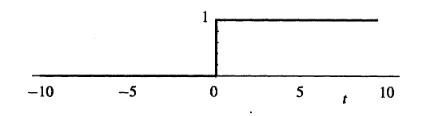
\includegraphics[width=0.8\textwidth]{img/pic9.png}}\\
      \subfloat[The current response.]{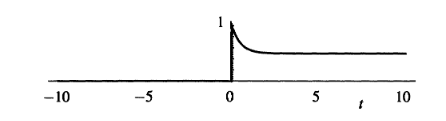
\includegraphics[width=0.8\textwidth]{img/pic8.png}}  
    \end{figure}
  \end{column}
  \end{columns}
\end{frame}

% SLIDE 4
\begin{frame}{Example of Grey Box Model}
  \begin{columns}
    \begin{column}{0.5\textwidth}
      \begin{tcolorbox}[width=1\linewidth, height = 1.1\linewidth]
      \textbf{Stochastic Models}
      \begin{align*}
        dx_t &= f(x_t, u_t, t, \theta) + \sigma(u_t, t, \theta)d\omega \\
        y_k  &= h(x_k, u_k, t_k, \theta) + e_k
      \end{align*}
    
      Suitable for both linear, non-linear models.  
      Used to represent systems influenced by both deterministic and stochastic components,
      accounting for random fluctuations in the system and uncertainties. \\
      \textbf{CTSM-R} is a great R package from DTU Compure to fit \textit{sde}.
      \end{tcolorbox}\pause 

    \end{column}
    \begin{column}{0.5\textwidth}
      \begin{tcolorbox}[width=1\linewidth, height = 1.1\linewidth]
        \textbf{PINNs:Physics-informed neural networks} \\
        Gaining attention in recent years, as a class of machine learning techniques that combine data-driven neural
        networks with physical equations to solve complex problems in various fields,
        such as physics, and engineering, minimizing the discrepancy between the predictions made by the neural network and physical equations.
        \end{tcolorbox}
    \end{column}
\end{columns} 



\end{frame}

% SLIDE 5
\begin{frame}{Example of Black Box Models}
  A black box model is a system or algorithm that makes predictions or decisions based solely on input and output data,
  without an interpretable framework that can explain the connection between the inputs and the outputs.
  \begin{figure}
    \centering
    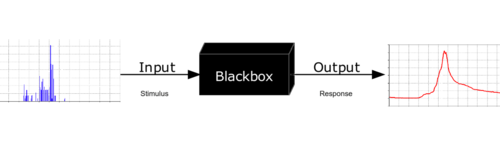
\includegraphics[scale=0.5]{img/pic10.png}
    \caption{Caption for the Image}
    \label{fig:example}
  \end{figure}

\end{frame}

% SLIDE 6
\begin{frame}{AutoRegressive Model (\textbf{AR})}
\begin{block}{Test}
  Let's consider the simplest form of an AR model:
  \begin{equation*}
    y_{t} = a y_{t-1} + \epsilon
  \end{equation*}
\end{block}
  Where $y_{k-1}$ is the value of the time series at time $t-1$ and $\epsilon$ an error term. 
  \begin{block}{General}
    \begin{equation*}
      y_{k} = a_{1}y_{t-1} + a_{2}y_{t-2} + \dots + a_{n}y_{t-n} + \epsilon_t = \sum_{i=1}
    \end{equation*}
  \end{block}
\end{frame}

% SLIDE 7
\begin{frame}{AutoRegressive eXogenous Model (\textbf{ARX})}
  \begin{block}{}
    Given an \textbf{LTI} system, with $\bm{y_t}$ the output signal \textit{with exogenous} input $\bm{u_t}$ with delay \textit{k}, an ARX model can be defined as follows:
    \begin{align*}
      y(t) = c + a_{1}y(t-1) + \dots + a_{n_a}y(t-n_a) + \\ 
              + b_{1}u(t-n_k) + \dots + b_{n_b}u(t-n_k-n_b-1) + \epsilon(t)      
    \end{align*}
    Or in a more compact form: 
    \begin{align*}
      y(t) = \varphi'\theta + \epsilon(t)
    \end{align*}

  Where $\phi$ is the regressor vector, $\theta$ is the paramters vector to estimate, and  (white noise process). 
  \end{block}
  \end{frame}

  % SLIDE 8
  \begin{frame}{AutoRegressive eXogenous Model (\textbf{ARX})}
    \begin{block}{Test}
      Given an LTI system, with $y_t$ the output signal with exogenous input $u_t$ of delay k, an ARX model can be defined as follows:
      \vspace{1em}
      \begin{align*}
        \boxed{y(t) = \varphi'\theta + \epsilon(t)}
      \end{align*}
    \begin{align*}
      \bm{\theta} &= [a_1, \dots, a_{n_a} \; b_1, \dots, b_{n_b}]' \\
      \bm{\varphi}(t) &= [y(t-1), \dots, y(t-n_a) \quad u(t-n_k) \dots, u_{t-n_k-n_b+1}]' \\
      \bm{\epsilon}(t) &\sim \mathcal{N}(0,\sigma^2)
    \end{align*}
    \end{block}
    \end{frame}

% SLIDE 9
\begin{frame}{Paramters Estimation}
    \begin{block}{}
    Therefore, for a SISO (Single Input Single Output) time series, $y_{t+1}$ can be written as: 
    \begin{align*}
      \hat{y}(t+1|\theta) = \varphi(t+1)'\theta
    \end{align*}  
    
  \end{block}
\end{frame}

% SLIDE 10
\begin{frame}{}
    \begin{columns}
    \column{0.5\textwidth} 
    
\includegraphics[width=0.5\textwidth]{img/pic5.png} \centering \pause
    
    \column{0.5\textwidth} % Second column

    \begin{itemize}
      \item $\varphi$' is the regressor vector 
      \item $\epsilon(t)$ is the error \pause
      \item $\theta$ is the coefficients vector (to be estimated)
    \end{itemize}
    \end{columns}
\end{frame}

% SLIDE 11
\begin{frame}{Parameters Estimation}
      \begin{block}{}
        We don't know $\theta$ yet, but we have collected a set $Z^N$ of measured data.
        \begin{align*}
          Z^N = \{u(-n), y(-n)\dots u(N-1), y(N-1) \}, \: n = max\{n_a,n_{b}+n_{k}-1\}
        \end{align*}
      Therefore, we use the \textcolor{red}{least squared error} to find the optimal paramters vector $\theta^*$ that minimize the prediction error between $\hat{y}(t+1|\theta)$ and $y(t)$, namely: 
      \begin{align*}
        \theta^* = \underset{\theta}{\text{arg\;min}} \{\mathcal{L}(\theta, Z^N)\}
      \end{align*}
      \begin{align*}
        \mathcal{L}(\theta, Z^N) = \frac{1}{N}\sum_{k=0}^{N-1}(y(k)-\hat{y}(t|\theta))^2 = \frac{1}{N}\sum_{k=0}^{N-1}(y(k)-\varphi'(t)\theta)^2 
      \end{align*}
    \end{block}
\end{frame}

% SLIDE 12
\begin{frame}{Paramters Estimation}
  \begin{block}{}
      $\mathcal{L}(\theta, Z^N)$ is a quadratic function of $\theta$. Therefore, $\theta^*$ can be found by zeroing The derivative of $\mathcal{L}$.
  \begin{align*}
    \frac{d}{d\theta} \mathcal{L}_N(\theta, Z^N) = \frac{2}{N}\sum_{k=0}^{N-1}\varphi(t)(y(k)-\varphi'(t)\theta)  = 0 
  \end{align*}
Thus, obtaining: 
\begin{align*}
  \sum_{k=0}^{N-1}\varphi(t)y(k) = \sum_{k=0}^{N-1}\varphi(t)\varphi'(k)
\end{align*}
Finally, the $\theta^*$ can be derived: 
\begin{center}
    \begin{align*}
      \boxed{\theta^* = \Biggr[\sum_{k=0}^{N-1}\varphi(t)\varphi'(t)\Biggr]^{-1} \: \Biggr[\sum_{k=0}^{N-1}\varphi(t)y(t)\Biggr]}
    \end{align*}
\end{center}
\end{block}
\end{frame}

% SLIDE 13
\begin{frame}{Paramters Estimation}
  \begin{block}{}
    Thus, obtaining: 
\begin{align*}
  \sum_{k=0}^{N-1}\varphi(t)y(k) = \sum_{k=0}^{N-1}\varphi(t)\varphi'(k)
\end{align*}
Finally, $\theta^*$ can be derived: 
\begin{center}
\begin{tcolorbox}[width=0.6\linewidth, height = 0.22\linewidth, colframe=red]
    \begin{align*}
      \theta^* = \Biggr[\sum_{k=0}^{N-1}\varphi(t)\varphi'(t)\Biggr]^{-1} \: \Biggr[\sum_{k=0}^{N-1}\varphi(t)y(t)\Biggr]
    \end{align*}
\end{tcolorbox}
\end{center}
\end{block}
\end{frame}

% SLIDE 14
\begin{frame}[fragile]{\small{Generate SISO data}}
  \begin{minted}[fontsize=\scriptsize]{python}
def generate_siso_data(n, noise_level=0.1, a1=0.5, a2=-0.3, b1=0.7, b2=-0.2):
    """
    Generates synthetic Single Input Single Output (SISO) data for an ARX model with na=2 and nb=2.
    :param n: Number of data points to generate.
    :param noise_level: Standard deviation of the noise.
    :param a1, a2: Coefficients for the autoregressive part of the model.
    :param b1, b2: Coefficients for the exogenous input part of the model.
    :return: Tuple of (y, x), where y is the target series and x is the exogenous series.
    """
    # Generating exogenous input (x) as a pseudo-binary random signal
    x = np.random.randint(0, 2, size=n)

    # Generating the target series (y)
    y = np.zeros(n)
    for t in range(2, n):
        y[t] = a1 * y[t-1] + a2 * y[t-2] +
               b1 * x[t-1] + b2 * x[t-2] + np.random.normal(0, noise_level)

    return y, x
  \end{minted}
\end{frame}

% SLIDE 15
\begin{frame}[fragile]{Visualize the data}
  \begin{minted}[fontsize=\scriptsize]{python}
    y, x = generate_siso_data(n=100, noise_level=0.05)
  \end{minted}
  \begin{figure}
    \centering
    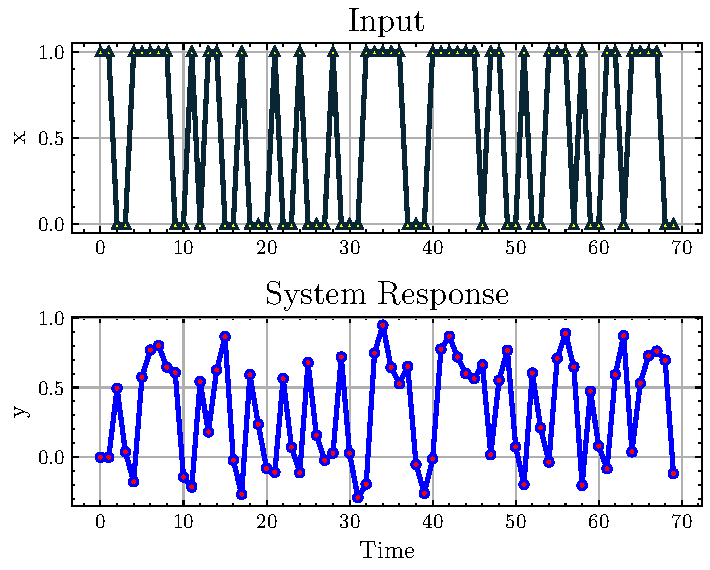
\includegraphics[width=0.55\textwidth]{img/response.pdf}
    \label{fig:your-plot}
  \end{figure}
\end{frame}

% SLIDE 16
\begin{frame}[fragile]{\small{Fit an ARX Model}}
  \begin{minted}[fontsize=\scriptsize]{python}
def fit_arx_model(y, x, na, nb):
    """
    :param y: Target time series.
    :param x: Exogenous time series.
    :param na: Order of the autoregressive part.
    :param nb: Order of the exogenous input part.
    :return: Coefficients of A, B and the intercept of the ARX model.
    """
    max_lag = max(na, nb)
    features = []
    target = y[max_lag:]

    for i in range(max_lag, len(y)):
        lag_y = y[i-na:i] if na > 0 else []
        lag_x = x[i-nb:i] if nb > 0 else []
        row = np.concatenate([lag_y, lag_x])
        features.append(row)

    X = np.array(features)
    model = LinearRegression().fit(X, target)
    return model.coef_[:na], model.coef_[na:], model.intercept_
  \end{minted}
\end{frame}

% SLIDE 17
\begin{frame}[fragile]{\small{Estimated Paramters}}
  \begin{minted}[fontsize=\scriptsize]{python}
  na, nb = 2, 2
  coefficients_a, coefficients_b, intercept = fit_arx_model_with_intercept(y, x, na, nb)
  \end{minted}

  \begin{table}
    \centering
  \begin{tabular}{|l|c|}
      \toprule
      \textbf{Regressors} & \textbf{Parameters} \\
      \midrule
      intercept        & \num{0.0035} \\
      $x(t-1)$ & \num{0.7112} \\
      $x(t-2)$ & \num{-0.2089} \\
      $y(t-1)$ & \num{0.5071} \\
      $y(t-2)$ & \num{-0.3255} \\
      \bottomrule
    \end{tabular}
  \end{table}
  \vspace{1em}\pause
  Are these parameters similar to the ones previously defined?
\end{frame}

% SLIDE 18
\begin{frame}[fragile]{\underbar{SysIdentPy}: A Python for System identification}
  \href{https://github.com/wilsonrljr/sysidentpy}{\textcolor{blue}{SysIdentPy}} is a Python library designed for linear and non-linear system identification.
\begin{itemize}
  \item FROLS $\rightarrow$ Forward Regression Orthogonal Least Squares.
  \item Particularly effective in nonlinear system. 
  \item Itertively adding new terms to the model, creating a pool of candidate terms (linear, nonlinear) based on the input data.
  \item The orthogonalization process multicollinearity.
\end{itemize}
\end{frame}

% SLIDE 19
\begin{frame}[fragile]{\underbar{SysIdentPy}: A Python for System identification}
  In this example we test this library on our SISO system to fit an ARX fit, manually selecting the order of the model.
  
  \begin{minted}[fontsize=\scriptsize]{python}
    from sysidentpy.model_structure_selection import FROLS
    from sysidentpy.basis_function._basis_function import Polynomial

    basis_function = Polynomial(degree=1)

    model = FROLS(
        order_selection=False,
        n_terms=5,
        extended_least_squares=False,
        ylag=2,
        xlag=2,
        estimator="least_squares",
        basis_function=basis_function,
    )

    model.fit(X=x.reshape(-1,1), y=y.reshape(-1,1))
  \end{minted}
\end{frame}

% SLIDE 20
\begin{frame}
  \begin{columns}
    \begin{column}{0.5\textwidth}
      Estimated Coeff. Our Models \centering
      \begin{table}
        \centering
      \begin{tabular}{|l|c|}
          \toprule
          \textbf{Regressors} & \textbf{Parameters} \\
          \midrule
          intercept        & \num{0.0035} \\
          $x(t-1)$ & \num{0.7112} \\
          $x(t-2)$ & \num{-0.2089} \\
          $y(t-1)$ & \num{0.5071} \\
          $y(t-2)$ & \num{-0.3255} \\
          \bottomrule
        \end{tabular}
      \end{table}
    \end{column}

    \begin{column}{0.5\textwidth}
      Estimated Coeff. FROLS \centering
      \begin{table}
        \centering
      \begin{tabular}{|l|c|}
          \toprule
          \textbf{Regressors} & \textbf{Parameters} \\
          \midrule
          intercept        & \num{0.0115} \\
          $x(t-1)$ & \num{0.7034} \\
          $x(t-2)$ & \num{-0.1962} \\
          $y(t-1)$ & \num{0.4883} \\
          $y(t-2)$ & \num{-0.3367} \\
          \bottomrule
        \end{tabular}
      \end{table}
    \end{column}
  \end{columns}
\end{frame}

% SLIDE 21
\begin{frame}[fragile]{Forecast  using  \underbar{SysIdentPy}}
  \begin{minted}[fontsize=\scriptsize]{python}
    yhat = model.predict(X=x.reshape(-1,1), y=y.reshape(-1,1)).squeeze()
  \end{minted}
  \begin{figure}
    \centering
    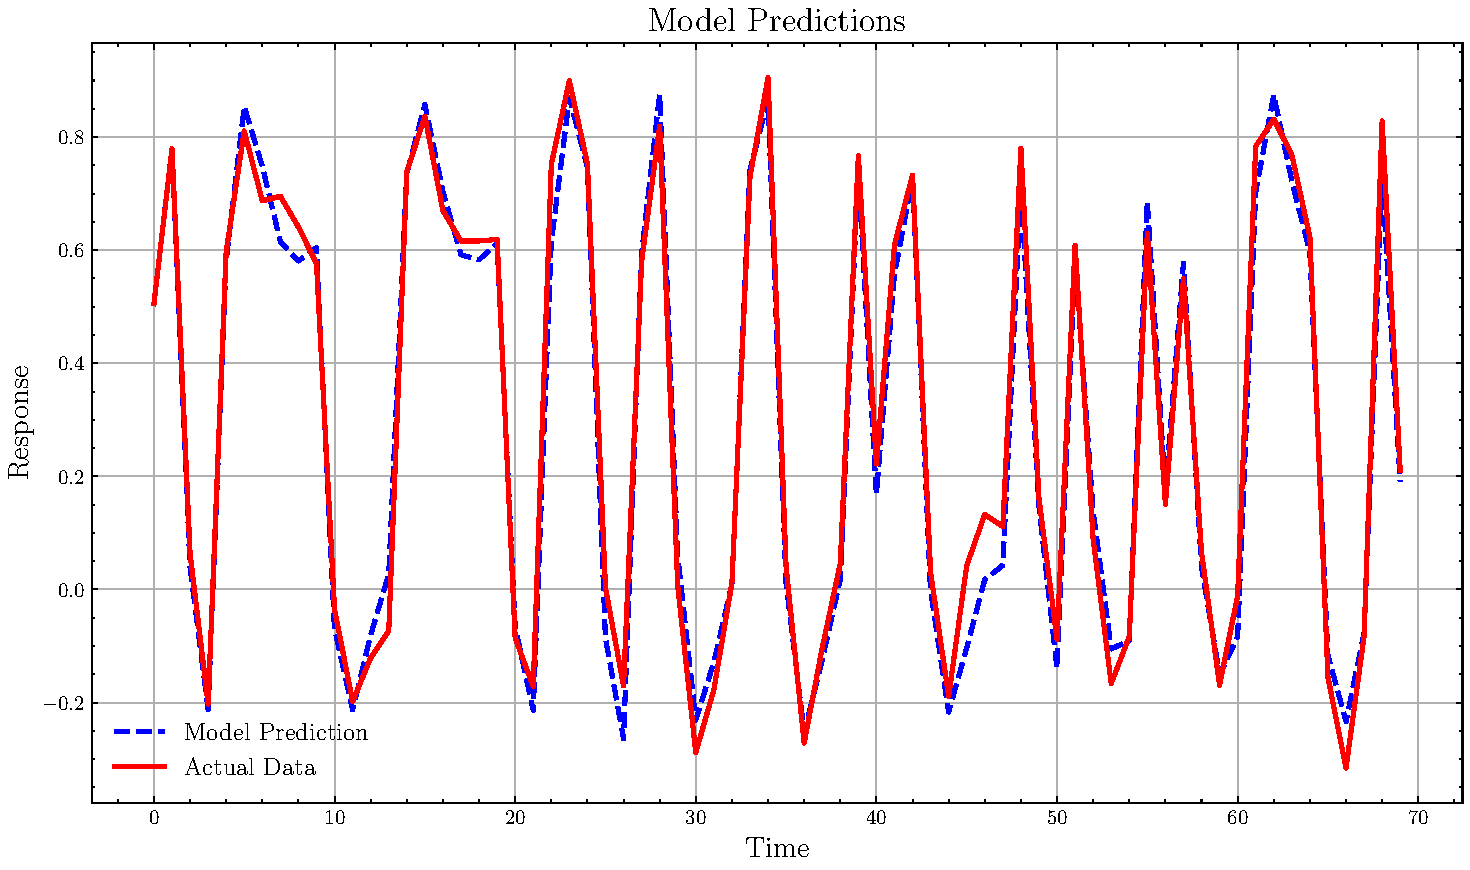
\includegraphics[width=0.6\textwidth]{img/response_yhat.pdf}
  \end{figure}
  
\end{frame}

% SLIDE 22
\begin{frame}[fragile]{RMSE: Root Mean Squared Error}
  \begin{equation}
      MSE = \frac{1}{n} \sum_{i=1}^{n} (y_i - \hat{y}_i)^2
  \end{equation}
  \begin{minted}[fontsize=\scriptsize]{python}
    from sklearn.metrics import mean_squared_error
    MSE = mean_squared_error(y, yhat) # Mean Squared Error
    RMSE = np.sqrt(MSE) #Root Mean Squared Error
  \end{minted}
\end{frame}

% SLIDE 23
\begin{frame}{}
  \begin{columns}
  \column{0.3\textwidth} 
  
\includegraphics[width=0.6\textwidth]{img/pic5.png} \centering
  
  \column{0.7\textwidth} % Second column
    \textbf{Do you rember the assumtion on} $\epsilon(t)$ \textbf{?} \centering \\
    \vspace{2em}
    We previously assumed that the residual of the model, namely $(y - \hat{y})$ 
    are distributed as $\epsilon(t)\sim \mathcal{N}(0,\sigma^2)$.
    \vspace{2em}

    In our example we have introduce a distrurbance modeled as gaussian noise with $\sigma = 0.01$
    If the model is good enough, we error will coincide with the gaussian noise we introduced.
  \end{columns}
\end{frame}

% SLIDE 24
\begin{frame}{Model Validation}
  \textbf{Shapiro-Wilk} test confirmed that the residuals are white noise and the Q-Q Plot below shows that the distribution of the residual is compatible with the noise introduced in our data $\sim \mathcal{N}(0,\sigma^2 = 0.05)$.
  \begin{figure}
    \centering
    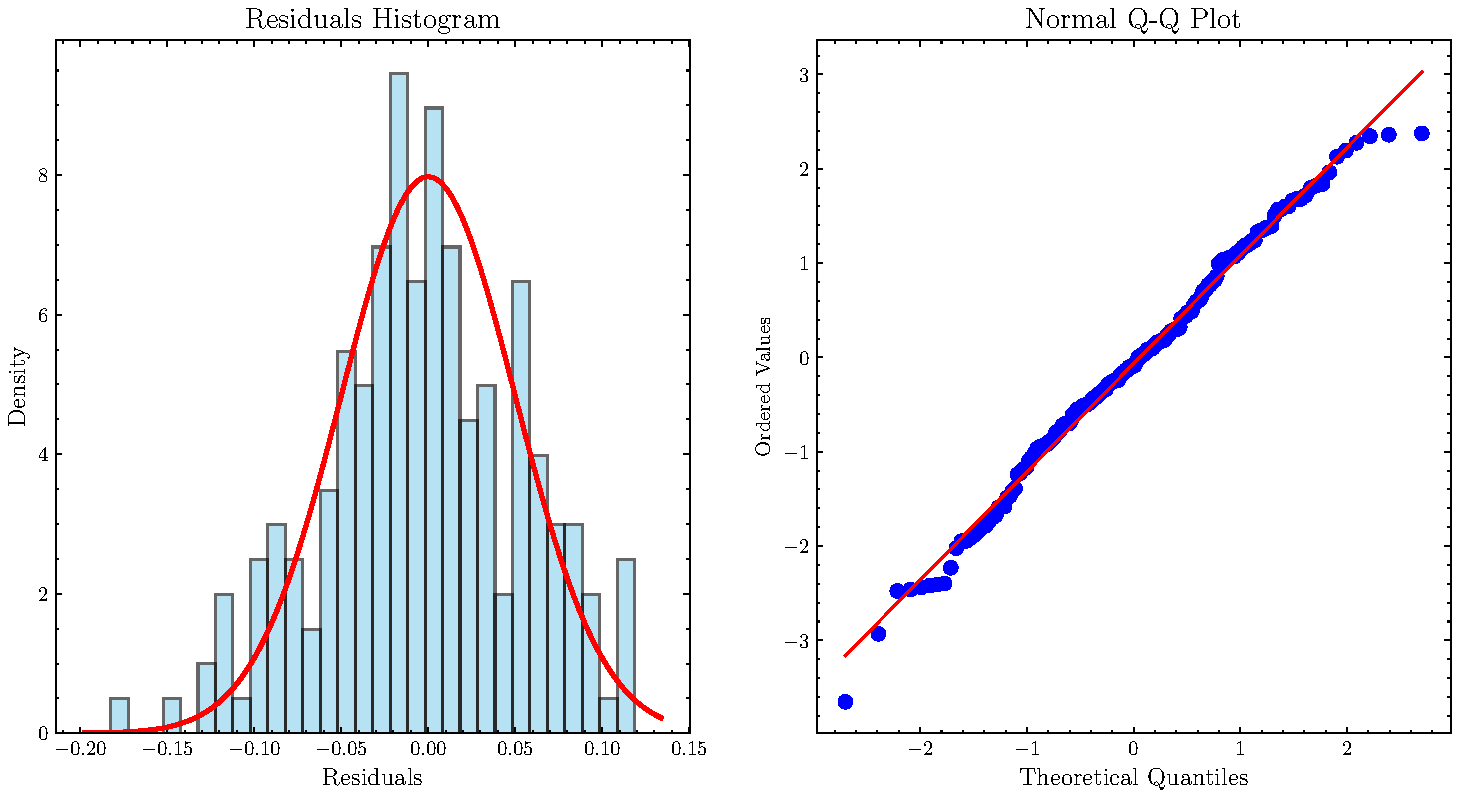
\includegraphics[width=0.7\linewidth]{img/residuals_analysis.pdf}
  \end{figure}
\end{frame}

% SLIDE 25
\begin{frame}{}
  \begin{columns}
  \column{0.3\textwidth} 
  
\includegraphics[width=0.6\textwidth]{img/pic5.png} \centering
  
  \column{0.7\textwidth} % Second column
    \textbf{Do you rember the assumtion on} $\epsilon(t)$ \textbf{?} \centering \\
    \vspace{2em}
    
  \end{columns}
\end{frame}

\end{document}